\documentclass[10pt]{exam}
\usepackage[utf8]{inputenc}

\usepackage[margin=1in]{geometry}
\usepackage{amsmath,amssymb}
\usepackage{multicol}
\usepackage{multirow}
\usepackage{graphicx}
\usepackage{tikz}
\newcommand{\clase}{CÁLCULO INTEGRAL}
\newcommand{\examnum}{Parcial 1}
\newcommand{\examdate}{20 de Febrero de 2020}
\newcommand{\timelimit}{120 Minutos}
\definecolor{Micolor1}{gray}{0.7}
\pagestyle{head}
\firstpageheader{\Large\sc\clase}{}{\sc\examnum}
\runningheader{\sc\clase}{}{\sc\examnum\ - Page \thepage\ of \numpages}
\runningheadrule


\begin{document}
\vspace{1.5cm}
\begin{tabular}{ll}
\multirow{5}{*}{
\includegraphics[scale=0.28]{Sabana1.png}}
%&\textbf{Examen Final}\\
& \large\hspace{0.5cm}Nombre: \makebox[2.7in]{\hrulefill}\vspace{0.2cm}\\
& \large\hspace{0.5cm}Fecha:\textbf{\examdate} \vspace{0.2cm}\\
& \large\hspace{0.5cm}Tema: A \vspace{0.2cm}\\
& \large\hspace{0.5cm}Profesor: \makebox[2.7in]{\hrulefill}\vspace{0.2cm}\\
%& \large\hspace{1.0cm}Tiempo límite: \textbf{\timelimit}}
\end{tabular}\\
\rule[2ex]{\textwidth}{2pt} 
\begin{itemize}
\scriptsize{\item \textbf{No se permite el uso de elementos electrónicos, smartwatches, etc. La presencia de cualquier equipo de comunicación en el entorno del examen es considerado intento de fraude. Éste o cualquier otro intento de fraude implica cero en el examen y se reporta a la facultad.}
    \item \textbf{La comprensión del examen es parte de la evaluación, por tanto, no se responden preguntas.} 
    \item \textbf{Se evalúa procedimiento y/o justificación, por tanto, sea claro y ordenado.}
   % \item \textbf{Este examen contiene \numpages\ páginas y \numquestions\ preguntas.  El Total de puntos en esta prueba es de \numpoints}
   }
\end{itemize} 

%\begin{center}
%\textbf{Tabla de Puntos (No marcar. Uso exclusivo del profesor)}\\
\addpoints
%\gradetable[v][questions]
%\end{center}

\noindent
\rule[2ex]{\textwidth}{2pt}


\begin{enumerate}
\normalsize
\setlength{\columnsep}{10mm}

    \item  \textbf{Flores Bogotá}
ha estimado que su ganancia (en millones de pesos) está dada por la función $F(x)$, donde $x$ es el número  (en miles) de flores producidas.



$$F(x)=\int_0^{x^2-8x}e^{-t}\, dt,\,\,\,\,\,\,\,\,\,t>0$$
\begin{enumerate}

    \item \textbf{[6 puntos]} ¿A qué razón cambiará la ganancia de la empresa cuando se producen 3000 flores ($x=3$)?  Deje su respuesta indicada.\hfill{[B2]} 
    \item \textbf{[8 puntos]} El Gerente de \textbf{Flores Bogotá}  ha manifestado que si se producen 3000 flores ($x=3$) la ganancia de su empresa aumentaría, ¿es esto cierto,  justifique?.
    Una función es creciente si su derivada es mayor que cero. \hfill{[B3]} 
    \item \textbf{[4 puntos]} ¿Cuál es el nivel de producción que \textbf{Flores Bogotá} deberá obtener si desea una ganancia máxima?  \hfill{[B3]}
    \end{enumerate}




   \item \textbf{[4 puntos]} Calcule $$\int \left(\dfrac{1}{\sqrt{x}}+\dfrac{1}{3x}+\sin{(a)}+2^x \right)\, dx$$ 
$a$ es constante. \hfill{[C1]}
\item Una heladería desea conocer la cantidad de helado que gasta en un cono, para esto, rotará alrededor del eje $x$ la siguiente figura.

\begin{center}
    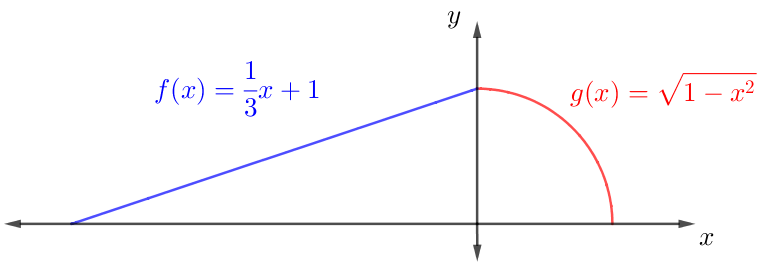
\includegraphics[scale=1.5]{cono.png}
\end{center}

\begin{enumerate}
   \item \textbf{[6 puntos]} Plantee la integral que representa la cantidad de helado que puede contener la  base (galleta) del cono (rotación de $f(x)$). \hfill{[B2]}

   \item \textbf{[6 puntos]} Plantee la integral que represente la cantidad de helado que puede contener la parte superior del cono (rotación de $g(x)$). \hfill{[B2]}
    
   \item \textbf{[4 puntos]} ¿Cuál es la cantidad de helado que puede contener el sólido resultante al rotar $f(x)$ y $g(x)$ alrededor del eje $x$?  \hfill{[B2]}
    
    
\end{enumerate}

\newpage
\item Considere la gráfica de la función $f(x)=x^2+1$

\begin{center}
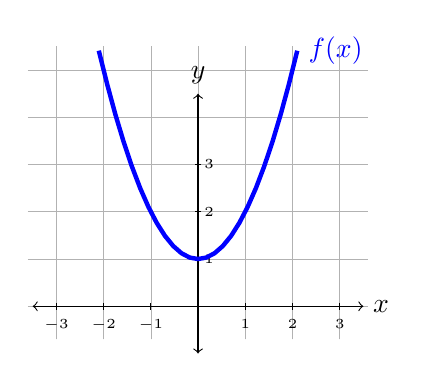
\begin{tikzpicture}[scale=0.6,domain=-2.1:2.1]
 \foreach \pos in {1,2}
\draw[very thin,color=Micolor1] (-3.6,-0.7) grid (3.6,5.5);
\draw[<->] (-3.5,0) -- (3.5,0) node[right] {$x$};
\foreach \pos in { -3, -2, -1,1, 2, 3}
\draw[shift={(\pos,0)}] (0pt,2pt)--(0pt,-2pt) node[below]{\tiny{$\pos$}};
\draw[<->] (0,-1) -- (0,4.5) node[above] {$y$};
\foreach \pos in {  1, 2, 3}
\draw[shift={(0,\pos)}] (2pt,0pt)--(-2pt,0pt) node[right]{\tiny{$\pos$}};

\draw[color=blue,ultra thick] plot (\x,\x*\x+1) node[right] {$f(x)$};
\end{tikzpicture}\\

\end{center}



\begin{enumerate}
    \item \textbf{[4 puntos]}  Halle una aproximación a la integral     $\displaystyle{\int_{-2}^{2}f(x)\, dx}$ usando una suma de Riemann con extremos de la izquierda y $n=4$.  Grafique los rectángulos del área de aproximación. \hfill{[C2]}

   

     \item \textbf{[4 puntos]} Utilice el teorema fundamental del cálculo para evaluar  $\displaystyle{\int_{-2}^{2}f(x)\, dx}$. \hfill{[C2]}
     
     \item \textbf{[6 puntos]} ¿Cuál  es el error de aproximación  que se obtiene del inciso (a)? \hfill{[C3]}
     

\end{enumerate}


 \item  \textbf{Polución}
En cierta localidad de Bogotá el nivel de ozono $ L(t) $ a las  7 am  es $0.25$ partes por millón (ppm). El pronóstico del clima para las siguientes 12 horas anuncia que el nivel de ozono  $t$ horas después de las 7:00 am  cambiará a la razón de:  
	
		
	$$L^{\prime}(t)=\dfrac{\frac{6}{25}-\frac{3t}{100}}{\sqrt{-t^2+16t+36}}$$
	partes por millón por hora (ppm/h).
	
	\begin{enumerate}
		
		\item \textbf{[6 puntos]} Expresar el nivel de ozono $L(t)$ como una función del tiempo $t$.   \hfill{[B2]} 
		\item \textbf{[4 puntos]} Determinar  el nivel de ozono a las 9:00 am
		\hfill{[B3]} 

	\end{enumerate}	
	
\item  \textbf{Demanda}
 La función de la demanda de una bicicleta para ejercicio que se vende exclusivamente en televisión por cable es: $p=d(x)=\dfrac{\sqrt{900-2x}}{10} $, donde p es el precio unitario en cientos de dólares y $x$ es la cantidad demandada por semana. La función de suministro correspondiente está dada por: $p=s(x)=\dfrac{\sqrt{100+2x}}{10}$ donde $p$ tiene el mismo significado que el anterior y $x$ es el número de bicicletas para ejercicio que el proveedor tendrá disponible al precio $p$.
 
 \begin{center}
    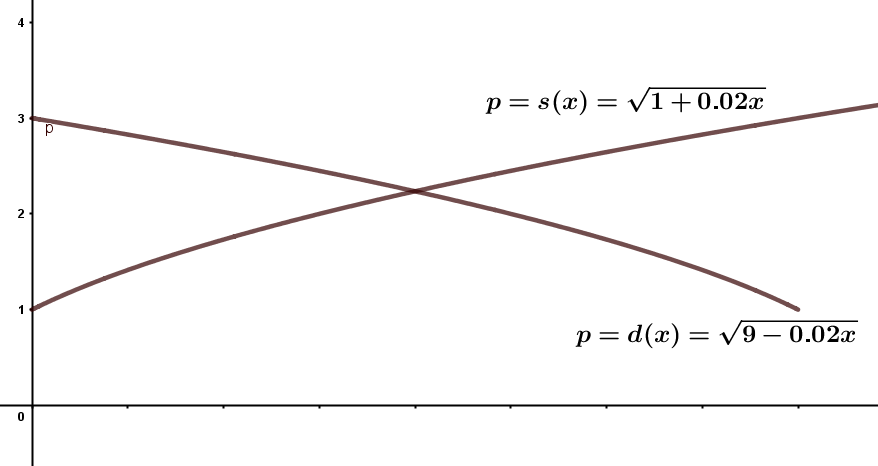
\includegraphics[scale=0.5]{demanda.PNG}
\end{center}
 
 	\begin{enumerate}
		
		\item \textbf{[4 puntos]} Determine el precio de equilibrio  \hfill{[B2]} 
		\item \textbf{[6 puntos]} Determiner el excedente de consumidor si el precio unitario es sostenido al precio de equilibrio.
		\hfill{[B2]} 

	\end{enumerate}	


\end{enumerate}




\end{document}
